\chapter{Results}
After extensive testing of different hyperparameters, the model that produced the best accuracy was used to predict the pixel class for the data in the test dataset that was left untouched during training. 
\section{Hyperparameters}
A simple grid search was used to iterate over a list of all possible combinations for the hyperparameters, train the model for 100 epochs on each and calculate the accuracy on the test dataset. The parameters chosen are shown in Table \ref{tab.grid_search}. 
\begin{table}[htbp]
\centering 
\begin{tabular}{l|l}
                           & \textbf{Possibilities}   \\ \hline
\textbf{Number of Filters} & 2, 4, 8, 16, 32, 64      \\ 
\textbf{Learning Rate}     & 0.1, 0.01, 0.001, 0.0001 \\ 
\textbf{Batch Size}        & 16, 12, 64, 128, 256     \\ 
\end{tabular}
\caption[Hyperparameter possibilities]{Depicts all the possibilities considered for the hyperparameters chosen in this study.}
\label{tab.grid_search}
\end{table}
\begin{figure}[htpb]
    \centering
    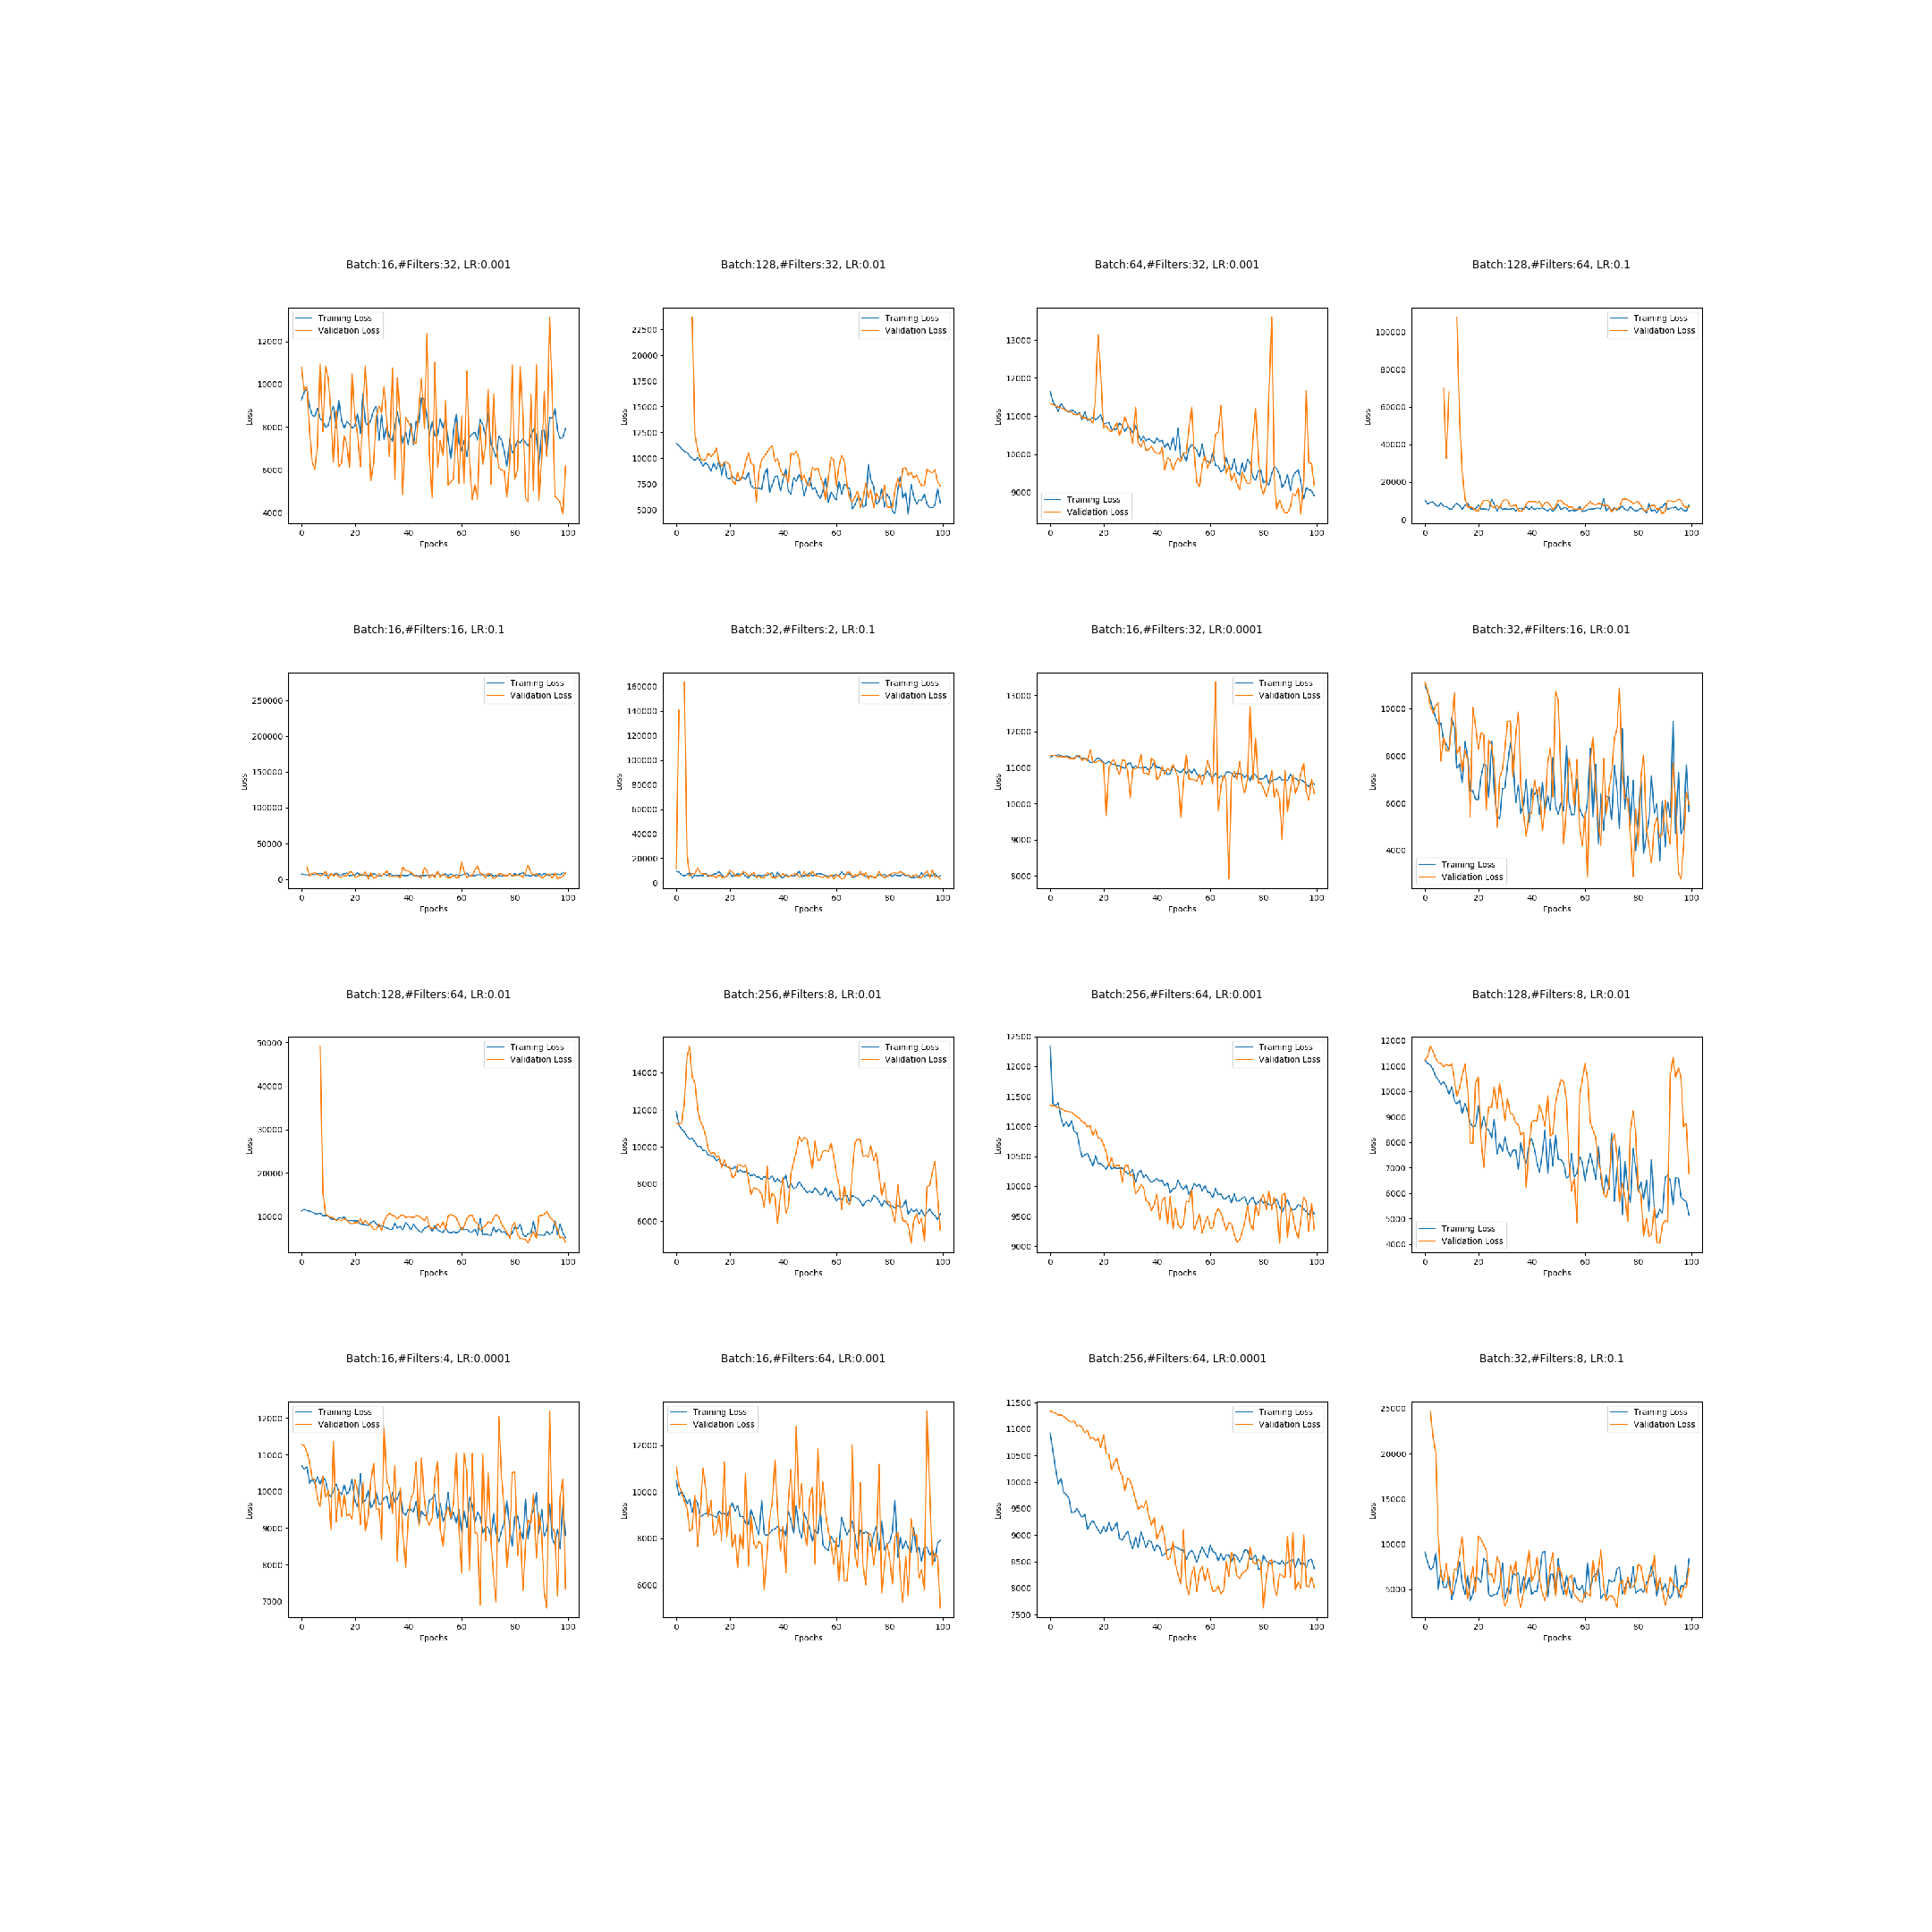
\includegraphics[width=\textwidth]{\dir/figs/hp_grid.png}
    \caption[Learning Rate Curves for Various Hyperparameter Combinations]{Learning rate curves for various hyperparameter combinations.}
    \label{fig.hyperparameters}
\end{figure}
\section{Accuracy}
Throughout the training process, the network saves the state of the weights and the biases whenever the loss rate reduces. This model state can then be loaded again at a later data and training can continue. The final stage of training, takes the model state that results in the lowest loss and applies it to the test data to make a prediction and evaluate the accuracy.
\section{Predictions}



